\documentclass[a4paper]{article}
\usepackage{fancyhdr}
\usepackage{lastpage}
\usepackage[utf8]{inputenc}
\usepackage[official]{eurosym}
\usepackage[left=2cm, right=2cm, top=2cm]{geometry} %right=30mm,left=30mm,top=15mm,bottom=20mm für die Bachelorarbeit/Seminararbeit
\usepackage{graphicx} % support the \includegraphics command and options
\usepackage{amsmath}
\usepackage{amssymb}
\usepackage{adjustbox}
\usepackage{mathtools}
\usepackage{centernot}
\usepackage{sectsty}
\usepackage[parfill]{parskip} % Activate to begin paragraphs with an empty line rather than an indent
\usepackage{booktabs} % for much better looking tables
\usepackage{array} % for better arrays (eg matrices) in maths
\usepackage{paralist}% very flexible & customisable lists (eg. enumerate/itemize, etc.)
\usepackage{verbatim} % adds environment for commenting out blocks of text & for better verbatim
\usepackage{subfig} % make it possible to include more than one captioned figure/table in a single float
\usepackage[table,xcdraw]{xcolor}
\usepackage{perpage}
\usepackage{hyperref}
\usepackage[perpage,symbol*]{footmisc}
\usepackage{chngcntr}
\usepackage{amsthm}
\usepackage{makecell}
\usepackage{csquotes}
\usepackage{lastpage}
\usepackage{tikz}
\usepackage{pgfplots}
\usepackage{framed}
\usepgfplotslibrary{fillbetween}
\usetikzlibrary{patterns}
\subsectionfont{\itshape}
\makeatletter
\renewcommand{\@seccntformat}[1]{}
\makeatother
\allowdisplaybreaks
\linespread{1.1}
\pagestyle{fancy}
\fancyhf{}
\lhead{Project I: One-Sector Growth Model} % add others
\rhead{Page \thepage \hspace{1pt} of \pageref{LastPage}}
\chead{Project II}
\title{Dynamic Macroeconomics with Numerics: Project II}
\author{Hashem Zehi, Samuel (120112285)\\Kotiers, Róza (11945569)\\Polzin, Julian (11948952)}
\date{\today}
\theoremstyle{definition}
\newtheorem{definition}{Definition}[section]
\newtheorem{lemma}{Lemma}[section]
\newtheorem{exmp}{Example}[section]
\newtheorem{note}{Note}[section]
\newtheorem{prop}{Proposition}[section]
\newcommand\Tau{\mathcal{T}}
\renewcommand{\thefootnote}{\fnsymbol{footnote}}
\newcommand*\diff{\mathop{}\!\mathrm{d}} %Integral d 
\newcommand\independent{\protect\mathpalette{\protect\independenT}{\perp}}
\def\independenT#1#2{\mathrel{\rlap{$#1#2$}\mkern2mu{#1#2}}}
\begin{document}
\maketitle
\newpage
\section{Part 1: Blanchard Kahn Approach}
First note that we have
	\begin{align*}
	z_{t+1} 	&= \exp(\epsilon_{t+1})z_{t}^{\rho} ,
	\intertext{but we may also use}
	z_{t+1} 	&= \exp( x_{t+1}) 	= \exp(\rho x_{t} + \epsilon_{t+1}),
	\end{align*}
Furthermore, we have from the Euler error defined in the last project two different capital utilization functions, differing only in the exponent
	\begin{align*}
	U_{t+1}^{\alpha} 	&= \Big( \frac{\alpha}{\delta\phi} \Big)^{\frac{\alpha}{\phi-\alpha}} \exp\Big(\frac{(1-\alpha)\alpha}{\phi-\alpha}x_{t+1}\Big)k_{t+1}^{\frac{(\alpha-1)\alpha}{\phi-\alpha}} \\
	U_{t+1}^{\phi} 		&= \Big( \frac{\alpha}{\delta\phi} \Big)^{\frac{\phi}{\phi-\alpha}} \exp\Big(\frac{(1-\alpha)\phi}{\phi-\alpha}x_{t+1}\Big)k_{t+1}^{\frac{(\alpha-1)\phi}{\phi-\alpha}}
	\end{align*}
We have a \textbf{three-equation system}, having already plugged the values for $U_t, U_{t+1}$ given by	
	\begin{align*}
	\mathbf F(\mathbf s_{t+1},\mathbf s_{t}) = 
		\begin{pmatrix}
		(1) \\ (2) \\ (3)
		\end{pmatrix},	
	\end{align*}	
with the elements being given by the equations below:
\small
	\begin{align}
	c_{t+1}-\beta c_{t} \bigg[\alpha \exp\Big( \big[1-\alpha+\frac{(1-\alpha)\alpha}{\phi-\alpha} \big] x_{t+1} \Big) k_{t+1}^{\alpha-1+\frac{(\alpha-1)\alpha}{\phi-\alpha}}\Big( \frac{\alpha}{\delta\phi}\Big)^{\frac{\alpha}{\phi-\alpha}}+1-\delta \Big( \frac{\alpha}{\delta\phi}\Big)^{\frac{\phi}{\phi-\alpha}}k_{t+1}^{\frac{(\alpha-1)\phi}{\phi-\alpha}}\exp\Big(x_{t+1}\frac{(1-\alpha)\phi}{\phi-\alpha}\Big) \bigg]
	\end{align}
	\begin{align}
	\exp\Big( \Big[ 1-\alpha+\frac{(1-\alpha)\alpha}{\phi-\alpha} \Big]x_{t} \Big)k_{t}^{\alpha+\frac{(\alpha-1)\alpha}{\phi-\alpha}} \Big( \frac{\alpha}{\delta\phi}\Big)^{\frac{\alpha}{\phi-\alpha}}+k_{t}-\delta \Big( \frac{\alpha}{\delta\phi}\Big)^{\frac{\phi}{\phi-\alpha}}\exp\Big( \frac{(1-\alpha)\phi}{\phi-\alpha}x_{t} \Big)k_{t}^{1+\frac{(\alpha-1)\phi}{\phi-\alpha}}-c_{t}-k_{t+1}
	\end{align}
	\begin{align}
	x_{t+1} - \rho x_{t}
	\end{align}
\normalsize	
Now we take the partial derivatives w.r.t.\ $c_{t},c_{t+1},k_{t},k_{t+1},x_{t},x_{t+1}$ for all three equations evaluated at the steady state. First the Euler error partial derivatives evaluated at the steady state:
	\begin{align*}
	\frac{\partial}{c_{t}}(1) 		&= -\beta\bigg[\alpha  k_{*}^{\alpha-1+\frac{(\alpha-1)\alpha}{\phi-\alpha}}\Big( \frac{\alpha}{\delta\phi}\Big)^{\frac{\alpha}{\phi-\alpha}}+1-\delta \Big( \frac{\alpha}{\delta\phi}\Big)^{\frac{\phi}{\phi-\alpha}}k_{*}^{\frac{(\alpha-1)\phi}{\phi-\alpha}} \bigg] \\
	\frac{\partial}{k_{t}}(1) 		&= 0\\
	\frac{\partial}{x_{t}}(1) 		&= 0\\
	\frac{\partial}{c_{t+1}}(1) 	&= 1\\			
	\frac{\partial}{k_{t+1}}(1) 	&= -\beta c_{*} \bigg[\alpha \Big( \alpha-1+\frac{(\alpha-1)\alpha}{\phi-\alpha} \Big) k_{*}^{\alpha-2+\frac{(\alpha-1)\alpha}{\phi-\alpha}}\Big( \frac{\alpha}{\delta\phi}\Big)^{\frac{\alpha}{\phi-\alpha}}-\delta \Big( \frac{\alpha}{\delta\phi}\Big)^{\frac{\phi}{\phi-\alpha}}k_{*}^{\frac{(\alpha-1)\phi}{\phi-\alpha}-1}\Big( \frac{(\alpha-1)\phi}{\phi-\alpha}\Big) \bigg]\\
	\frac{\partial}{x_{t+1}}(1) 	&= -\beta c_{*}\bigg[\alpha \big[1-\alpha+\frac{(1-\alpha)\alpha}{\phi-\alpha} \big] k_{*}^{\alpha-1+\frac{(\alpha-1)\alpha}{\phi-\alpha}}\Big( \frac{\alpha}{\delta\phi}\Big)^{\frac{\alpha}{\phi-\alpha}}-\delta \Big( \frac{\alpha}{\delta\phi}\Big)^{\frac{\phi}{\phi-\alpha}}k_{*}^{\frac{(\alpha-1)\phi}{\phi-\alpha}}\frac{(1-\alpha)\phi}{\phi-\alpha} \bigg]
	\end{align*}
Now the law of motion for capital's partial derivatives evaluated at the steady state:
	\begin{align*}
	\frac{\partial}{c_{t}}(2) 		&= -1\\
	\frac{\partial}{k_{t}}(2) 		&= \Big( \alpha+\frac{(\alpha-1)\alpha}{\phi-\alpha} \Big)k_{*}^{\alpha-1+\frac{(\alpha-1)\alpha}{\phi-\alpha}} \Big( \frac{\alpha}{\delta\phi}\Big)^{\frac{\alpha}{\phi-\alpha}}+1-\delta \Big( \frac{\alpha}{\delta\phi}\Big)^{\frac{\phi}{\phi-\alpha}} \Big( 1+\frac{(\alpha-1)\phi}{\phi-\alpha} \Big) k_{*}^{\frac{(\alpha-1)\phi}{\phi-\alpha}} \\
	\frac{\partial}{x_{t}}(2) 		&= \Big[ 1-\alpha+\frac{(1-\alpha)\alpha}{\phi-\alpha} \Big]k_{*}^{\alpha+\frac{(\alpha-1)\alpha}{\phi-\alpha}} \Big( \frac{\alpha}{\delta\phi}\Big)^{\frac{\alpha}{\phi-\alpha}}-\delta \Big( \frac{\alpha}{\delta\phi}\Big)^{\frac{\phi}{\phi-\alpha}}\frac{(1-\alpha)\phi}{\phi-\alpha}k_{*}^{1+\frac{(\alpha-1)\phi}{\phi-\alpha}} \\
	\frac{\partial}{c_{t+1}}(2) 	&= 0\\			
	\frac{\partial}{k_{t+1}}(2) 	&= -1\\
	\frac{\partial}{x_{t+1}}(2) 	&= 0
	\end{align*}	
And lastly the error term from the law of motion for $x$'s partial derivatives evaluated at the steady state:
	\begin{align*}
	\frac{\partial}{c_{t}}(3) 		&= 0 \\
	\frac{\partial}{k_{t}}(3) 		&= 0 \\
	\frac{\partial}{x_{t}}(3) 		&= -\rho \\
	\frac{\partial}{c_{t+1}}(3) 	&= 0 \\			
	\frac{\partial}{k_{t+1}}(3) 	&= 0 \\
	\frac{\partial}{x_{t+1}}(3) 	&= 1
	\end{align*}
We have the two matrices
	\begin{align*}
	D \mathbf F_1(\cdot) = \begin{pmatrix} \frac{\partial}{\partial c_{t}}(1) & \frac{\partial}{\partial k_t}(1) & \frac{\partial}{\partial x_t}(1) \\ \frac{\partial}{\partial c_{t}}(2) & \frac{\partial}{\partial k_t}(2) & \frac{\partial}{\partial x_t}(2) \\ \frac{\partial}{\partial c_{t}}(3) & \frac{\partial}{\partial k_t}(3) & \frac{\partial}{\partial x_t}(3)  \end{pmatrix},\
	D \mathbf F_2(\cdot) = \begin{pmatrix} \frac{\partial}{\partial c_{t+1}}(1) & \frac{\partial}{\partial k_{t+1}}(1) & \frac{\partial}{\partial x_{t+1}}(1) \\ \frac{\partial}{\partial c_{t+1}}(2) & \frac{\partial}{\partial k_{t+1}}(2) & \frac{\partial}{\partial x_{t+1}}(2) \\ \frac{\partial}{\partial c_{t+1}}(3) & \frac{\partial}{\partial k_{t+1}}(3) & \frac{\partial}{\partial x_{t+1}}(3)  \end{pmatrix}
	\end{align*}
Due to the complexity of the following operation we do not provide any detailed analytical description, but it follows that we have the Jacobian of the state space given by
	\begin{align*}
	\mathbf J = - D \mathbf F_2(\mathbf s_*,\mathbf s_*)^{-1} D \mathbf F_1(\mathbf s_*,\mathbf s_*)
	\end{align*}
The result is a 3$\times$3 matrix. We then proceed in the exact same way as we did in the fourth and fifth exercise session, so any details beyond the policy functions are omitted. 

\textit{Note:} our policy function is written to match the dynare output, so we take deviations as the input.
	

\newpage
\subsection{(d) IRFs}
	\begin{figure}[!h]
	\centering
	\caption{(i): $\phi = 1.5,\ \delta = 0.0285,\ \rho = 0.9$}
	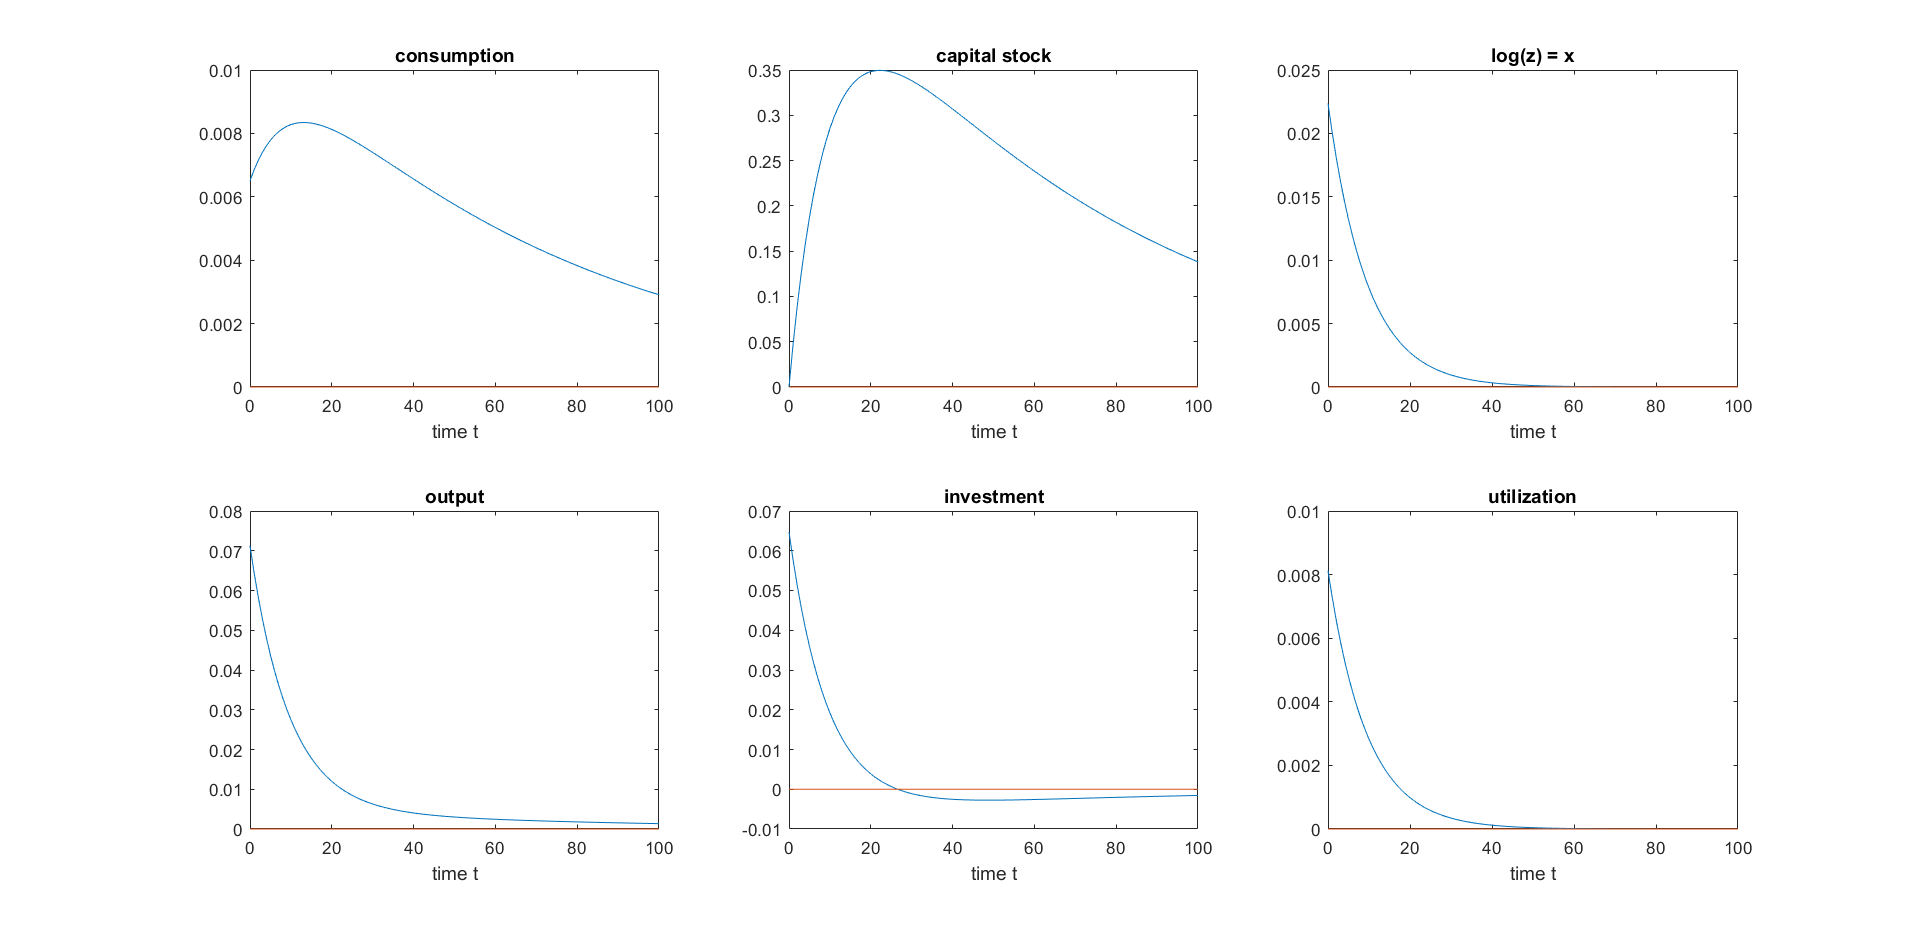
\includegraphics[width=\textwidth]{param1.png}
	\end{figure}
	\begin{figure}[!h]
	\centering
	\caption{(ii): $\phi = 1.5,\ \delta = 0.9,\ \rho = 0.9$}
	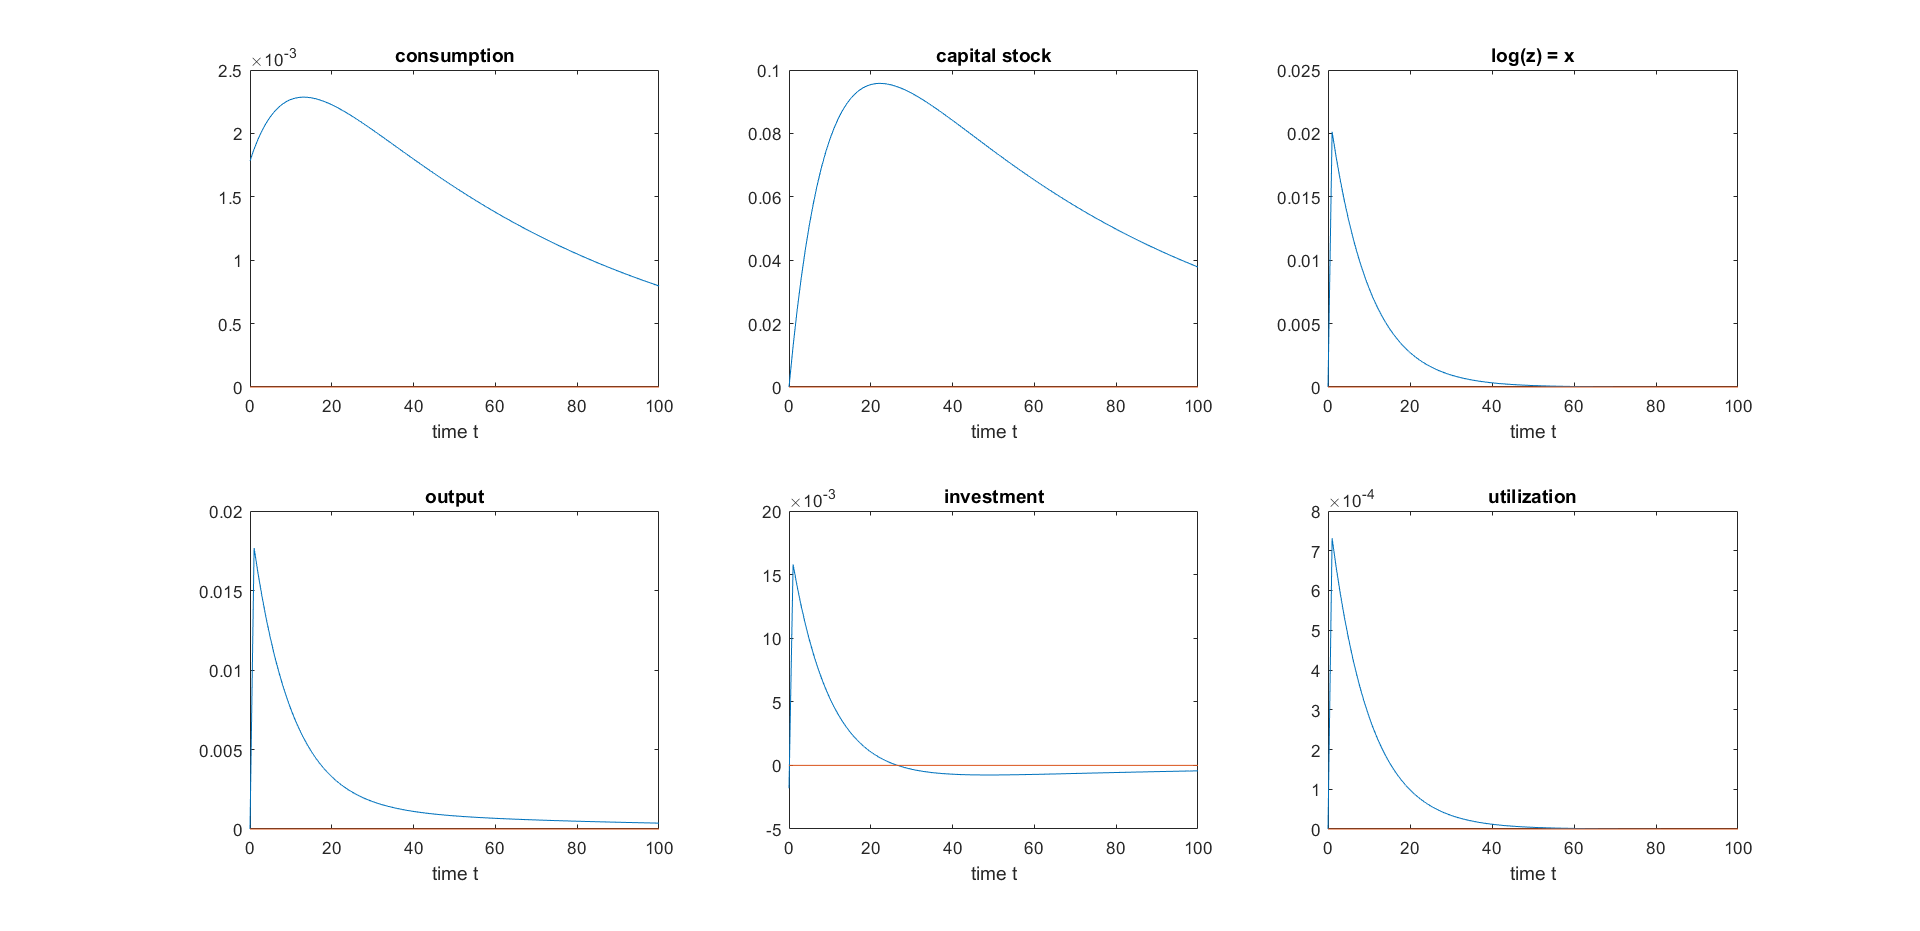
\includegraphics[width=\textwidth]{param2.png}
	\end{figure}
		\begin{figure}[!h]
	\centering
	\caption{(iii): $\phi = 1.5,\ \delta = 0.0285,\ \rho = 0.99$}
	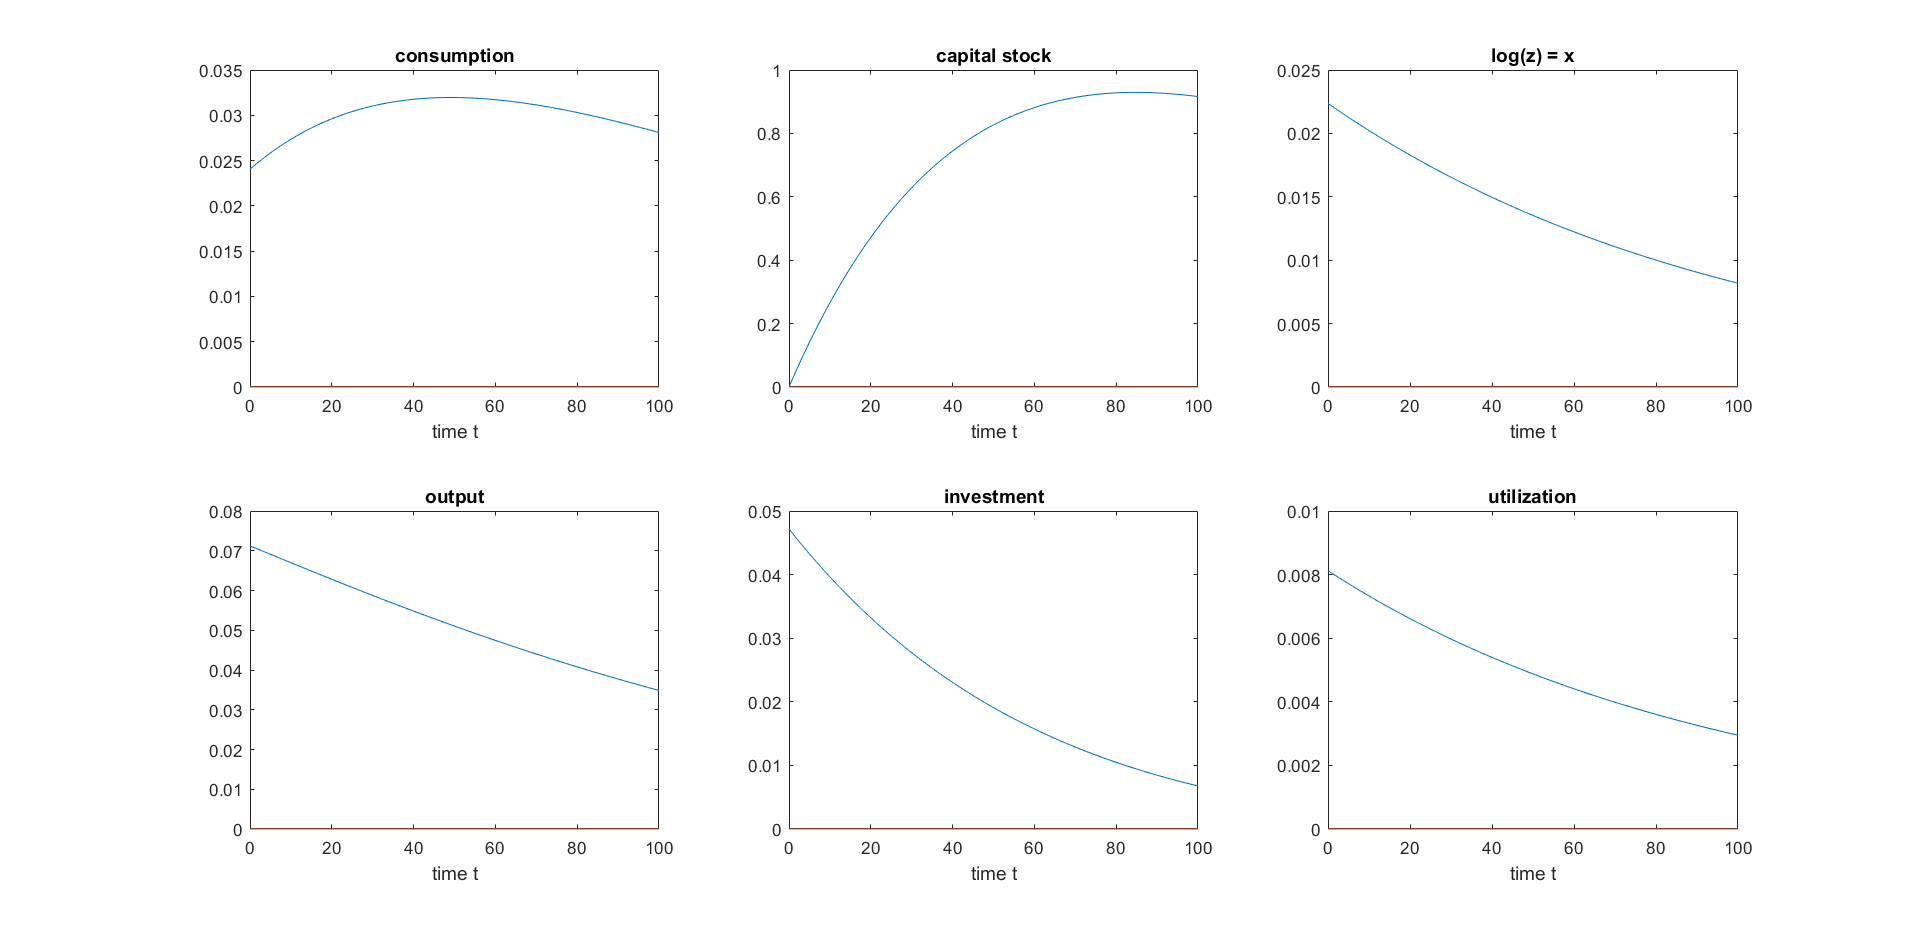
\includegraphics[width=\textwidth]{param3.png}
	\end{figure}
		\begin{figure}[!h]
	\centering
	\caption{(iv): $\phi = 1.1,\ \delta = 0.0285,\ \rho = 0.9$}
	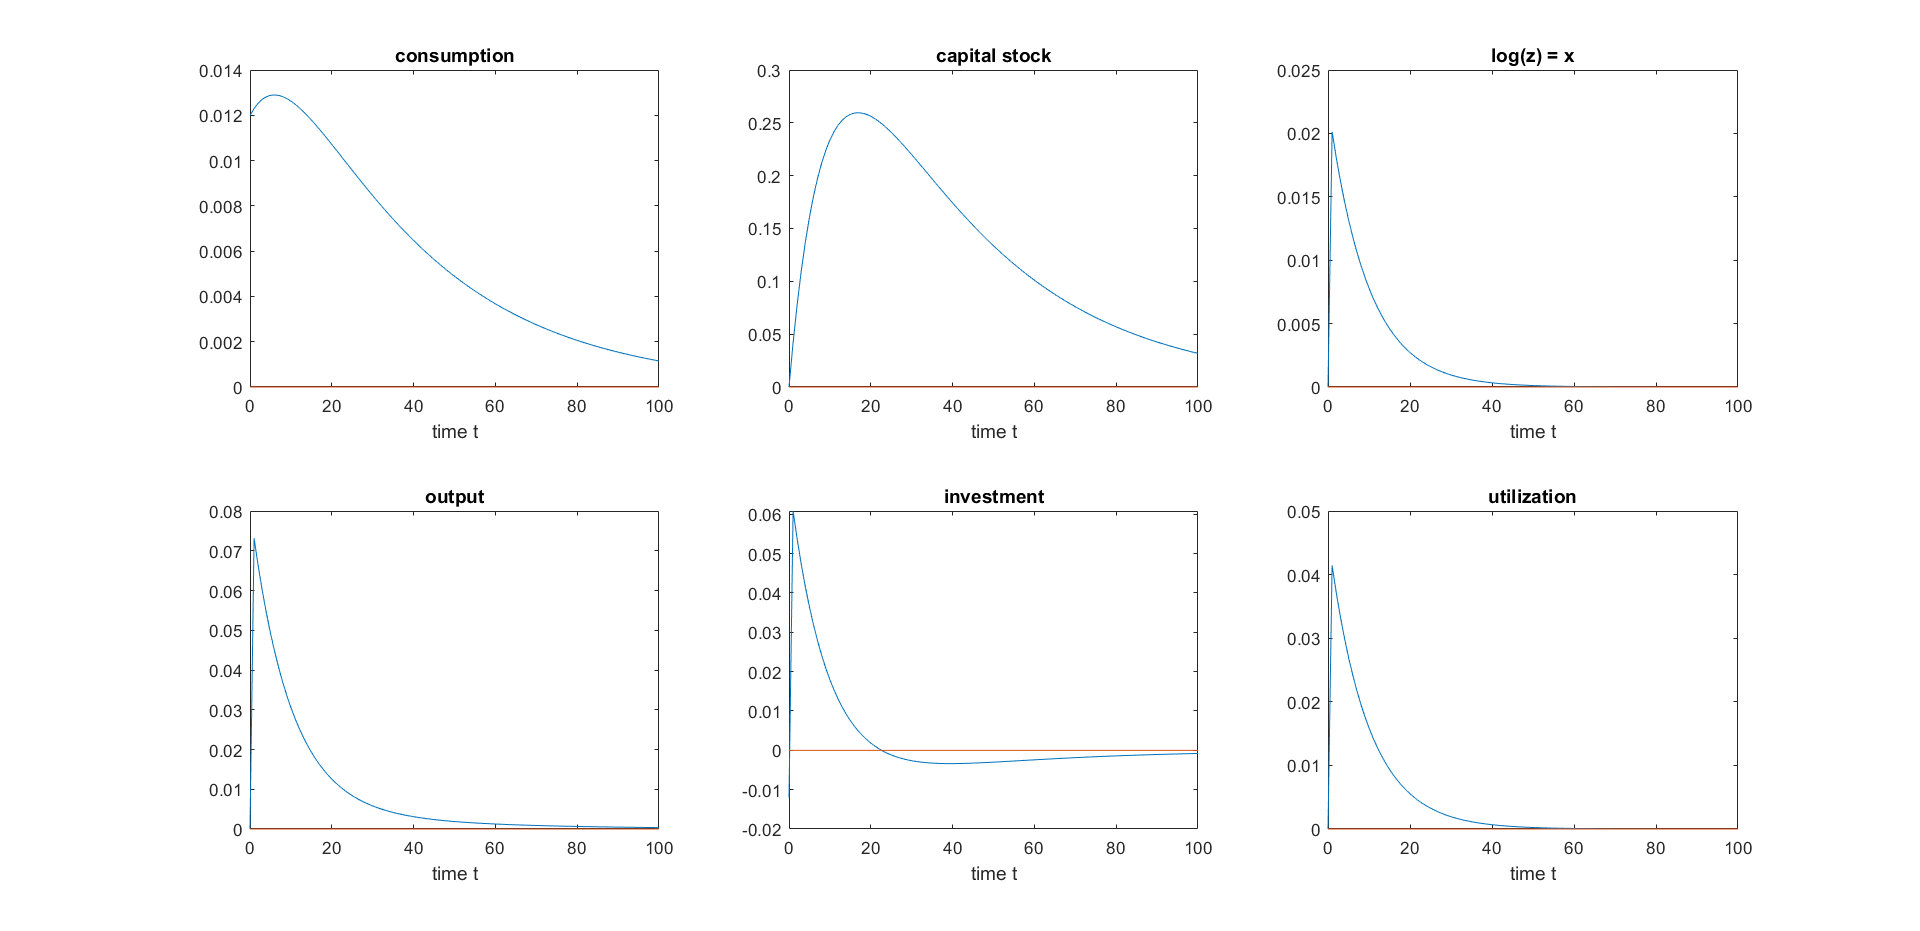
\includegraphics[width=\textwidth]{param4.png}
	\end{figure}


















\end{document}